\newpage
\section{Segmentação de Imagens}
O processo de segmentação de imagens é uma área que pertence a categorias maiores de visão computacional e processamento digital de imagens, sendo que esta possui como objetivo principal a distinção de áreas ou propriedades desejadas \cite{Haralick1985, Yuheng2017ImageOverview, Ghosh2019} de um determinado \textit{frame}, assim, sendo possível realizar análises mais precisas ou separar apenas as áreas que são convenientes e de interesse, de acordo com o objetivo da análise.

A partir de segmentações de imagens é possível realizar tarefas de reconhecimento, que são muito utilizadas para áreas de reconhecimento facial \cite{Yuheng2017ImageOverview}. Além dessa, dentre outras as grandes áreas para a aplicação das técnicas de segmentação de imagens, destacam-se setores da medicina, pavimentações, pedestres, carros autônomos, sensoriamento remoto e afins. Para exemplificar, as figuras \ref{segment:fig:1}\subref{segment:fig:1.1} e \ref{segment:fig:1}\subref{segment:fig:1.2} representam segmentações faciais e médicas, respectivamente.  

\begin{figure}[H]
   \caption{Exemplos de segmentações de imagens.}
   \centering
   \label{segment:fig:1}
    \begin{subfigure}[t]{0.5\textwidth}
        \centering
        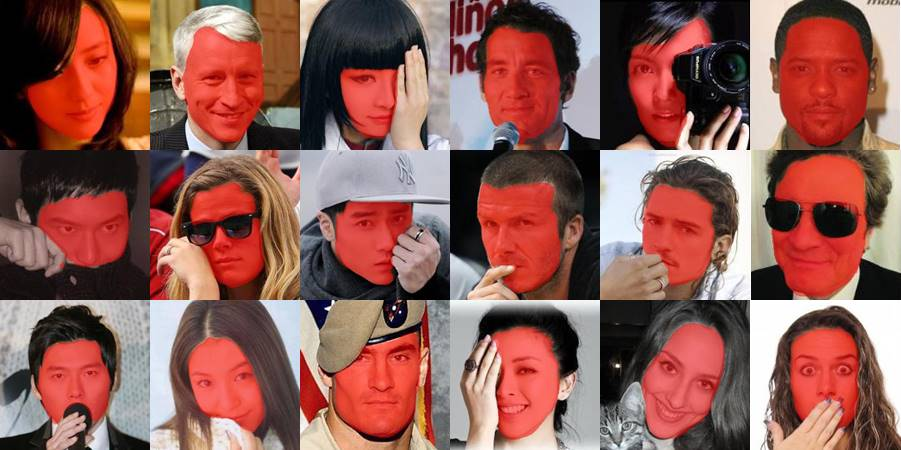
\includegraphics[width=1\linewidth]{recursos/imagens/image_seg/faces.png}
        \caption{Segmentação de imagens faciais.}
        \label{segment:fig:1.1}
    \end{subfigure}%
    ~ 

    \begin{subfigure}[t]{0.5\textwidth}
        \centering
        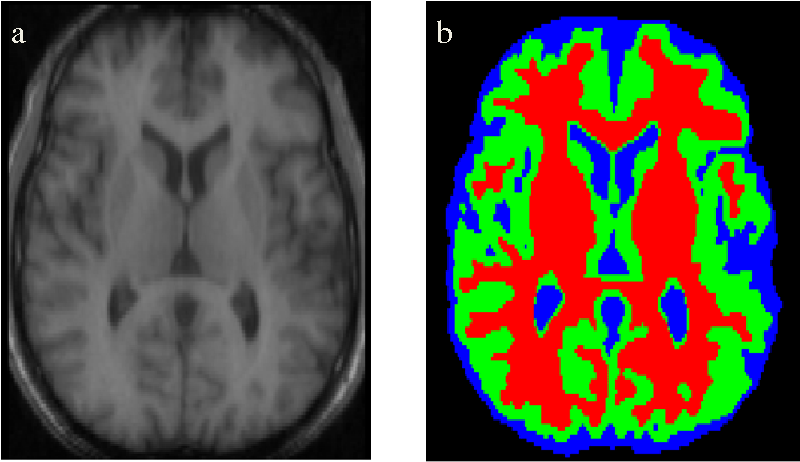
\includegraphics[width=1\linewidth]{recursos/imagens/image_seg/cerebro.png}
        \caption{Segmentação de imagem médica.}
        \label{segment:fig:1.2}
    \end{subfigure}%
    ~

    \vspace*{1 cm}
    Fonte: \cite{Nirkin2018OnPerception} e \cite{Withey2008ASoftware}, respectivamente.
\end{figure}

Assim, estando claro o conceito de segmentação de imagens, diversas técnicas são estudadas nessa área, tendo que os tradicionais serão citados na seção \ref{segment:segment}.


\subsection{Métodos e Técnicas Tradicionais}
\label{segment:segment}
\subsubsection{Segmentação Baseada em Regiões}

Alguns tipos de segmentação comumente trabalham com a os valores dos pixeis, de modo que seja possível segregar áreas e regiões de interesse de regiões que não são possuem relevância. Dentre as diversas técnicas, vale destacas a técnica de \textbf{\textit{Threshold Segmentation}}, ou em português, segmentação limiar, a qual é desenvolvida e aplicada em diversos trabalhos \cite{Yanowitz1989}.

De um modo geral a segmentação por meio da determinação de um limiar acontece em imagens/\textit{frames} que utilizam a escala de cinza ou algum sistema de cor que possua um canal voltado para intensidade, como o sistema HSV \cite{schneider2003experimentos}, visto que quando no sistema correto, há a determinação de um valor entre a o fundo e a área de interesse da imagem. Dessa forma, os pixeis acima do valor médio determinado são categorizados como área de intensidade e os inferiores são categorizados como fundo \cite{pedrini2008analise}, como é possível observar na equação \ref{segment:eq:1}, em que $T$ representa o limiar determinado, $f(x,y)$ o pixel da imagem $f$ e $g(x,y)$ o pixel limiarizado.

\begin{equation}
\label{segment:eq:1}
    g(x,y) = \left\{\begin{matrix}
        0, & se & f(x,y) \leq T\\ 
        1, & se & f(x,y) > T
    \end{matrix}\right.
\end{equation}

Sobre \textit{Threshold Segmentation}, vale citar que há uma série de técnicas para determinar o valor de limiarização como é trabalhado por \cite{Al-amri2010ImageTechniques}, mas habitualmente utiliza-se da média \cite{Al-amri2010ImageTechniques, Yanowitz1989, Yuheng2017ImageOverview} ou de técnicas adaptativas que são citadas em trabalhos, como \cite{Yanowitz1989}, mas que ganham repercussões abrangentes e é evidenciada na técnica Otsu \cite{Otsu1979THRESHOLDHISTOGRAMS.}, principalmente quando se trata de segmentações com um limiar global como demonstra o histograma na figura \ref{segment:fig:2}\subref{segment:fig:2.1} e o exemplo prático na figura  \ref{segment:fig:3}\subref{segment:fig:3.3}. Todavia, quando as regiões de interesse estão divididas, faz-se necessário a divisão de limiares locais, como pode ser observado na figura do histograma \ref{segment:fig:2}\subref{segment:fig:2.2}, equação \ref{segment:eq:2} ou na figura \ref{segment:fig:3}\subref{segment:fig:3.4}.

\begin{equation}
\label{segment:eq:2}
    g(x,y) = \left\{\begin{matrix}
        v1, & se & f(x,y) \leq T \\ 
        v2, & se & T_1 < f(x,y) \leq T_2 \\
        v3, & se & f(x,y) > T_2
\end{matrix}\right.
\end{equation}

\begin{figure}[H]
   \caption{Histogramas de limiarizações.}
   \centering
   \label{segment:fig:2}
    \begin{subfigure}[t]{0.45\textwidth}
        \centering
        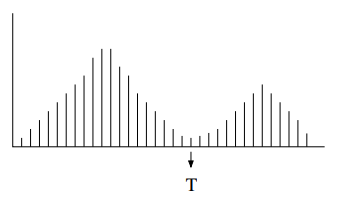
\includegraphics[width=0.5\linewidth]{recursos/imagens/image_seg/limi_glob.png}
        \caption{Histograma de limiarização global.}
        \label{segment:fig:2.1}
    \end{subfigure}%
    ~ 
    \begin{subfigure}[t]{0.45\textwidth}
        \centering
        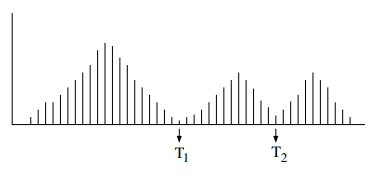
\includegraphics[width=0.5\linewidth]{recursos/imagens/image_seg/limi_local.png}
        \caption{Histograma de limiarização local.}
        \label{segment:fig:2.2}
    \end{subfigure}%

    \vspace*{1 cm}
    Fonte: retirado de \cite{pedrini2008analise}.
\end{figure}

\begin{figure}[H]
   \caption{Limiarizações.}
   \centering
   \label{segment:fig:3}
    \begin{subfigure}[t]{0.45\textwidth}
        \centering
        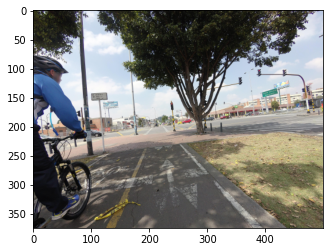
\includegraphics[height=1.5in]{recursos/imagens/image_seg/mapi.png}
        \caption{Imagem original.}
        \label{segment:fig:3.1}
    \end{subfigure}%
    ~ 
    \begin{subfigure}[t]{0.45\textwidth}
        \centering
        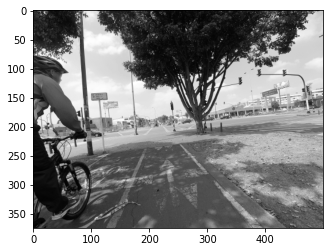
\includegraphics[height=1.5in]{recursos/imagens/image_seg/gray_mapi.png}
        \caption{Imagem em escala de cinza.}
        \label{segment:fig:3.2}
    \end{subfigure}%
    ~ 
    
    \begin{subfigure}[t]{0.45\textwidth}
        \centering
        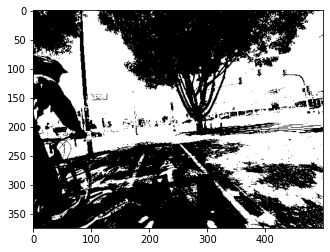
\includegraphics[height=1.5in]{recursos/imagens/image_seg/bw_mapi.png}
        \caption{Imagem limiarizada globalmente.}
        \label{segment:fig:3.3}
    \end{subfigure}
    ~
    \begin{subfigure}[t]{0.45\textwidth}
        \centering
        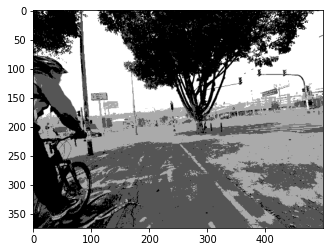
\includegraphics[height=1.5in]{recursos/imagens/image_seg/local_mapi.png}
        \caption{Imagem limiarizada localmente.}
        \label{segment:fig:3.4}
    \end{subfigure}

    \vspace*{1 cm}
    Fonte: retirado e adaptado de \cite{Neuhold2017_ICCV}.
\end{figure}

Por fim, ainda sobre a segmentação baseada em regiões, uma das técnicas que também se destaca é a de crescimento de regiões, ou em inglês, \textbf{\textit{Region Growning}}. Essa técnica consiste em traçar um limiar e distribuir sementes na imagem, de modo que os pixeis vizinhos sejam transformados pelo valor da semente quando com diferença inferiores ao limiar determinado, sendo possível visualizar tal ocorrência a partir da figura \ref{segment:fig:4} ou por meio da equação \ref{segment:eq:3}, sendo $P(R)$ o predicado da região, $f(r,s)$ o pixel semente, e $f(x,y)$ o pixel vizinho ao da semente por vizinhança-8,.

\begin{figure}[H]
   \caption{Crescimento de região.}
   \centering
   \label{segment:fig:4}
    \begin{subfigure}[t]{0.45\textwidth}
        \centering
        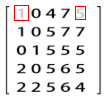
\includegraphics[height=1.5in]{recursos/imagens/image_seg/m1.png}
        \caption{Imagem original, sendo em vermelho os pixeis semente ($f(r,s)$).}
        \label{segment:fig:4.1}
    \end{subfigure}
    ~ 
    \begin{subfigure}[t]{0.45\textwidth}
        \centering
        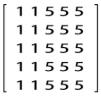
\includegraphics[height=1.5in]{recursos/imagens/image_seg/m2.png}
        \caption{Crescimento de região com $T = 3$.}
        \label{segment:fig:4.2}
    \end{subfigure}
    ~ 

    \begin{subfigure}[t]{0.45\textwidth}
        \centering
        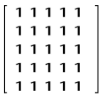
\includegraphics[height=1.5in]{recursos/imagens/image_seg/m3.png}
        \caption{Crescimento de região com $T = 6$.}
        \label{segment:fig:4.3}
    \end{subfigure}

    \vspace*{1 cm}
    Fonte: retirado e adaptado de \cite{Yuheng2017ImageOverview}.
\end{figure}

\begin{equation}
\label{segment:eq:3}
P(R) = \left\{\begin{matrix}
    VERDADEIRO, & se |f(x,y) - f(r,s)| \leq T \\
    FALSO,      &  caso\; contrario
\end{matrix}\right.
\end{equation}

Por fim, ainda sobre o aspecto de crescimento de região, salienta-se que é de extrema importância a determinação das sementes e do valor limiar \cite{Yuheng2017ImageOverview,pedrini2008analise}, assim como as condições para determinação de sistema de cores e canais são semelhantes as de \textit{threshold segmentation}.

\subsubsection{Segmentação por Bordas}
The edges can be considered as the discontinuous local features of an image.
Now the question is how can we detect these edges? This is where we can make use of filters and convolutions. as quais foram exploradas na seção \ref{deep:CNN}.
%%%%%%%%%%%%%%%%%%%%%%%%%%%%%%%%%%%%%%%%%%%%%%%%%%%%%%%%%%%%%%%%%%%%%%%%%%%%%%%%%%%%%%%%%%%%%%%%%%%%%
\begin{itemize}
    \item Citar sobel e laplacian (Olhar o livro do predini para poder citar);
    \item Colocar imagem de exemplo (https://colab.research.google.com/drive/1pnir$_$b3kSNHaycmmKgYzf8IOdOFbtOA6?usp=sharing) no final.
\end{itemize}
%%%%%%%%%%%%%%%%%%%%%%%%%%%%%%%%%%%%%%%%%%%%%%%%%%%%%%%%%%%%%%%%%%%%%%%%%%%%%%%%%%%%%%%%%%%%%%%%%%%%%

\subsubsection{Segmentação Baseada em Agrupamentos}
Clustering is the task of dividing the population (data points) into a number of groups, such that data points in the same groups are more similar to other data points in that same group than those in other groups. These groups are known as clusters.

Posto isso, destaca-se o uso do K-means \cite{macqueen1967some, bock2008origins}, o qual é um método não supervisionado que realiza agrupamento de dados de um \textit{dataset} de acordo com as suas similaridades e em quantidades desejadas ($k$). Ou seja, o algoritmo gera um ponto inicial randômico como centroide para um determinado \textit{cluster} e depois tenta atribuir os demais dados do \textit{dataset} aos \textit{clusters} de acordo com a sua proximidade. Para isso, o algoritmo usa técnicas de distância euclidiana \cite{Mahmud2012ImprovementAverage}. Vale ressaltar que os pontos centroides são atualizados conforme as classificações que são feitas no algoritmo, e os mesmos param de atualizar quando o algoritmo cumpre seu objetivo, há poucas interações dos dados com diferentes \textit{clusters} ou através de um número fixo de interações \cite{dunham2006data}.

Na imagem \ref{segment:fig:5} é possível observar o uso do algoritmo K-means para agrupar as regiões da imagem, tendo que foi definido um valor de $k = 3$.

\begin{figure}[H]
   \caption{Segmentação com K-means.}
   \centering
   \label{segment:fig:5}
    \begin{subfigure}[t]{0.45\textwidth}
        \centering
        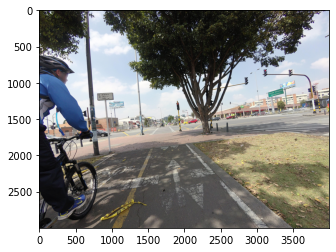
\includegraphics[height=1.5in]{recursos/imagens/image_seg/i1.png}
        \caption{Imagem original.}
        \label{segment:fig:5.1}
    \end{subfigure}%
    ~ 
    \begin{subfigure}[t]{0.45\textwidth}
        \centering
        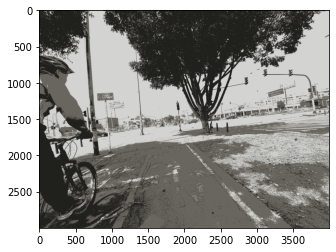
\includegraphics[height=1.5in]{recursos/imagens/image_seg/i2.png}
        \caption{Segmentação com $k = 3$.}
        \label{segment:fig:5.2}
    \end{subfigure}%

    \vspace*{1 cm}
    Fonte: retirado e adaptado de \cite{Neuhold2017_ICCV}.
\end{figure}


\subsubsection{Método \textit{Watershed}}

that can create a pixel-wise mask for each object in an image.
Mask R-CNN is an extension of the popular Faster R-CNN object detection architecture.
The Faster R-CNN method generates two things for each object in the image:
 - Its class
 - The bounding box coordinates
Mask R-CNN adds a third branch to this which outputs the object mask as well.
It also returns the mask for each proposal.
Mask R-CNN is the current state-of-the-art for image segmentation and runs at 5 fps.


\subsection{Considerações Finais da Seção}
Na seção \ref{segment:segment} foi comentado sobre os algoritmos comumente utilizados para segmentações mais simples, chegando no nível de complexidade de técnicas de \textit{machine learning} como o K-means.

Na tabela \ref{segment:table:1} é possivel visualizar as técnicas comentadas no decorrer da seção assim como uma breve descrição de seus usos, suas vantagens e desvantagens.

\begin{table}[!h]
    \centering
    \caption{Comparação entre os métodos tradicionais}
    \label{segment:table:1}
    \resizebox{\textwidth}{!}{
    \begin{tabular}{l|l|l|l}
    \textbf{Algoritmo}                  & \textbf{Descrição} & \textbf{Vantagens} & \textbf{Desvantagens} \\ \hline
    Segmentação Baseada em Regiões      &                    & Calculations are simpler, Fast operation speed, When the object and background have high contrast, this method performs really well          & When we don’t have significant grayscale difference, or there is an overlap of the grayscale pixel values, it becomes very difficult to get accurate segments. \\
    Segmentação por Bordas              &                    &                    &                       \\
    Segmentação Baseada em Agrupamentos &                    & The key advantage of using k-means algorithm is that it is simple and easy to understand. We are assigning the points to the clusters which are closest to them and k-means works really well when we have a small dataset. It can segment the objects in the image and give impressive results.                                               & But the algorithm hits a roadblock when applied on a large dataset (more number of images). It looks at all the samples at every iteration, so the time taken is too high. \\
    Método\textit{ Watershed}           &                    &                    &                                       
    \end{tabular}}
    
    \vspace*{1 cm}
    Fonte: autor.
\end{table}

Porém como comentado por \cite{Ghosh2019} e por \cite{Minaee2021} ...